\documentclass[a4paper, 12pt, final, garamond]{book}
\usepackage{cours-preambule}

\raggedbottom

\makeatletter
\renewcommand{\@chapapp}{\'Electrocin\'etique -- chapitre}
\makeatother

\toggletrue{student}
\HideSolutionstrue
\toggletrue{corrige}

\begin{document}
\setcounter{chapter}{6}

\chapter{\cswitch{Correction du TD}{TD~: filtrage lin\'eaire}}

\resetQ
\section{Filtrage et spectres}

\enonce{%
	Un signal périodique $e(t)$ (de fréquence \SI{1}{kHz}), dont le spectre est
	donné en figure 1, est envoyé à l'entrée de trois filtres différents. On
	effectue l'analyse spectrale du signal de sortie pour chaque filtre, les
	spectres obtenus sont donnés en figure 2, 3 et 4.

	\begin{center}
		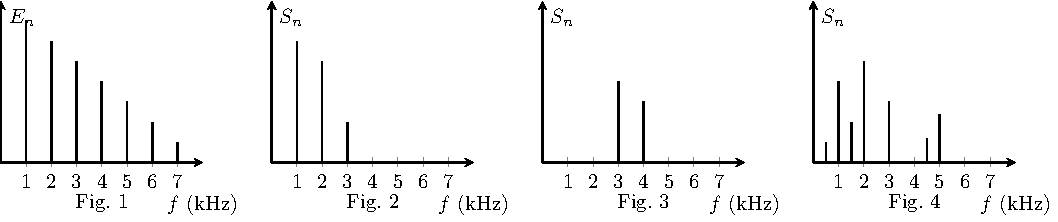
\includegraphics[width=\linewidth]{spectres_plain}
	\end{center}
}

\QR{%
	Quelles caractéristiques de chaque filtre peut-on déduire de ces spectres~?
}{%
	\begin{enumerate}
		\item Sur la figure deux, les basses fréquences sont globalement conservées,
		      et les fréquences à partir de \SI{3}{kHz} sont fortement atténuées voire
		      coupées~: \textbf{c'est un passe-bas}.
		\item Sur la figure trois, seules les fréquences entre 3 et \SI{4}{kHz} sont
		      gardées, les fréquences supérieures ou inférieures sont coupées~:
		      \textbf{c'est un passe-bande}.
		\item Sur la figure quatre, on ne distingue pas de relation simple vue en
		      cours~; on remarque de plus que de nouvelles fréquences apparaissent, ce
		      qui n'est pas le cas dans le filtrage linéaire~: c'est un \textbf{filtre
			      non-linéaire}.
	\end{enumerate}
}

\resetQ
\section{Filtre avec une bobine}
On considère le circuit ci-contre, avec $R = \SI{1.0}{k\Omega}$ et $L =
	\SI{10}{mH}$, donnant le diagramme de \textsc{Bode} ci-dessous~:
\smallbreak
\noindent
\begin{minipage}[c]{.49\linewidth}
	~
	\begin{center}
		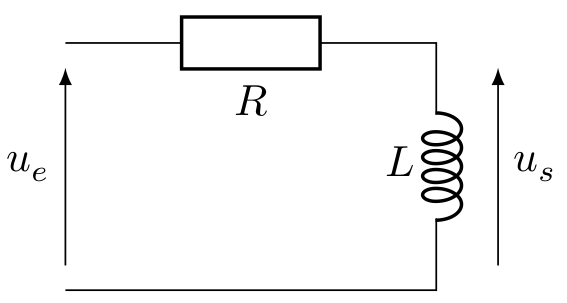
\includegraphics[width=\linewidth]{filtrebob_plain}
	\end{center}
\end{minipage}
\hfill
\begin{minipage}[c]{.49\linewidth}
	~
	\begin{center}
		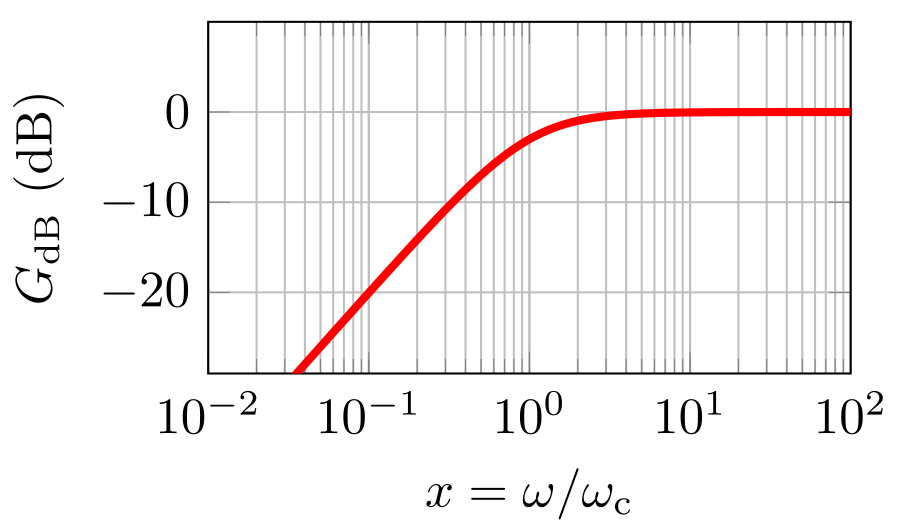
\includegraphics[width=\linewidth]{filtrebob_bode}
	\end{center}
\end{minipage}

\QR{%
	Sans utiliser le diagramme de \textsc{Bode}, quelle est la nature
	du filtre~?
}{%
	À basses fréquences, $\abs{\Zu_L} \opto{}{\w\ra0} 0$, donc
	$H(\w) \opto{}{\w\ra0} 0$. À hautes fréquences,
	$\abs{\Zu_L} \opto{}{\w\ra\infty} \infty$, donc
	$H(\w) \opto{}{\w\ra\infty} 1$~: \textbf{c'est un
		passe-haut}.
}

\QR{%
	Déterminer sa fonction de transfert et l'écrire sous la forme
	\[\Hu(\jw) = H_0 \frac{\jj\dfrac{\w}{\w_c}}{1 +
			\jj\dfrac{\w}{\w_c}}\]
	avec $H_0$ et $\w_c$ des constantes à préciser.
}{%
	On fait un pont diviseur de tension~:
	\begin{gather*}
		\xul{u_s} = \frac{\jlw}{R + \jlw}\xul{u_e}
		\Lra
		\frac{\xul{u_s}}{\xul{u_e}} = \Hu =
		\cancel{\frac{R}{R}}\times\frac{\jj\w\frac{L}{R}}{1 + \jj\w
			\frac{L}{R}}\\
		\Lra
		\boxed{\Hu(\jj\w) = H_0 \frac{\jj\frac{\w}{\w_c}}{1 +
				\jj\frac{\w}{\w_c}}}
		\qavec
		\boxed{H_0 = 1
			\qet
			\w_c = \frac{R}{L} = \SI{1e5}{rad.s^{-1}}}
	\end{gather*}
}

\QR{%
	Montrer par le calcul que la pente de l'asymptote du diagramme
	de \textsc{Bode} pour $\w \ll \w_c$ est de \SI{20}{dB/décade}.
}{%
	$1 + \jj \frac{\w}{\w_c} \underset{\w \ll \w_c}{\sim} 1$, et donc
	\begin{gather*}
		\Hu(\jj\w) \underset{\w\ll\w_c}{\sim} \jj \frac{\w}{\w_c}
		\Lra
		\boxed{G_{\rm dB} = 20\log \left( \abs{\Hu} \right)
			\underset{\w\ll\w_c}{\sim} 20\log x}
	\end{gather*}
	d'où la pente de \SI{20}{dB/décade}.
}

\QR{%
	On considère une tension d'entrée $u_e(t)$ somme de 3 harmoniques de
	mêmes amplitudes, de mêmes phases initiales, mais de fréquences
	respectives $f_1 = \SI{100}{Hz}$, $f_2 = \SI{1}{kHz}$ et $f_3 =
		\SI{100}{kHz}$. Donner le spectre de sortie.
}{%
	On trouve le spectre de sortie en multipliant chaque amplitude
	d'entrée par le module de la fonction de transfert pour avoir
	l'amplitude de sortie. \textbf{Attention, pulsation $\neq$ fréquence}.
	On a
	\[\abs{\Hu(f)} = \frac{\dfrac{2\pi f}{\w_c}}{\sqrt{1 +
				\left( \dfrac{2\pi f}{\w_c} \right)^2}}\]
	\begin{itemize}
		\item $H(f_1) \approx \num{6.3e-3}$~: le fondamental est
		      complètement atténué, il ne reste que \num{0.6}\% de son
		      amplitude initiale~;
		\item $H(f_2) \approx \num{6.3e-2}$~: l'harmonique $f_2$ est
		      fortement atténué, il n'en reste que 6\%~;
		\item $H(f_3) \approx \num{0.99}$~: l'harmonique $f_3$ est
		      pratiquement entièrement conservé.
	\end{itemize}
}

\resetQ
\section{Lecture de diagrammes de \textsc{Bode}}
\enonce{%
	On donne Figure~\ref{fig:ddBIII} les diagrammes de \textsc{Bode} de quatre
	filtres.
	\begin{figure}[htbp!]
		\centering
		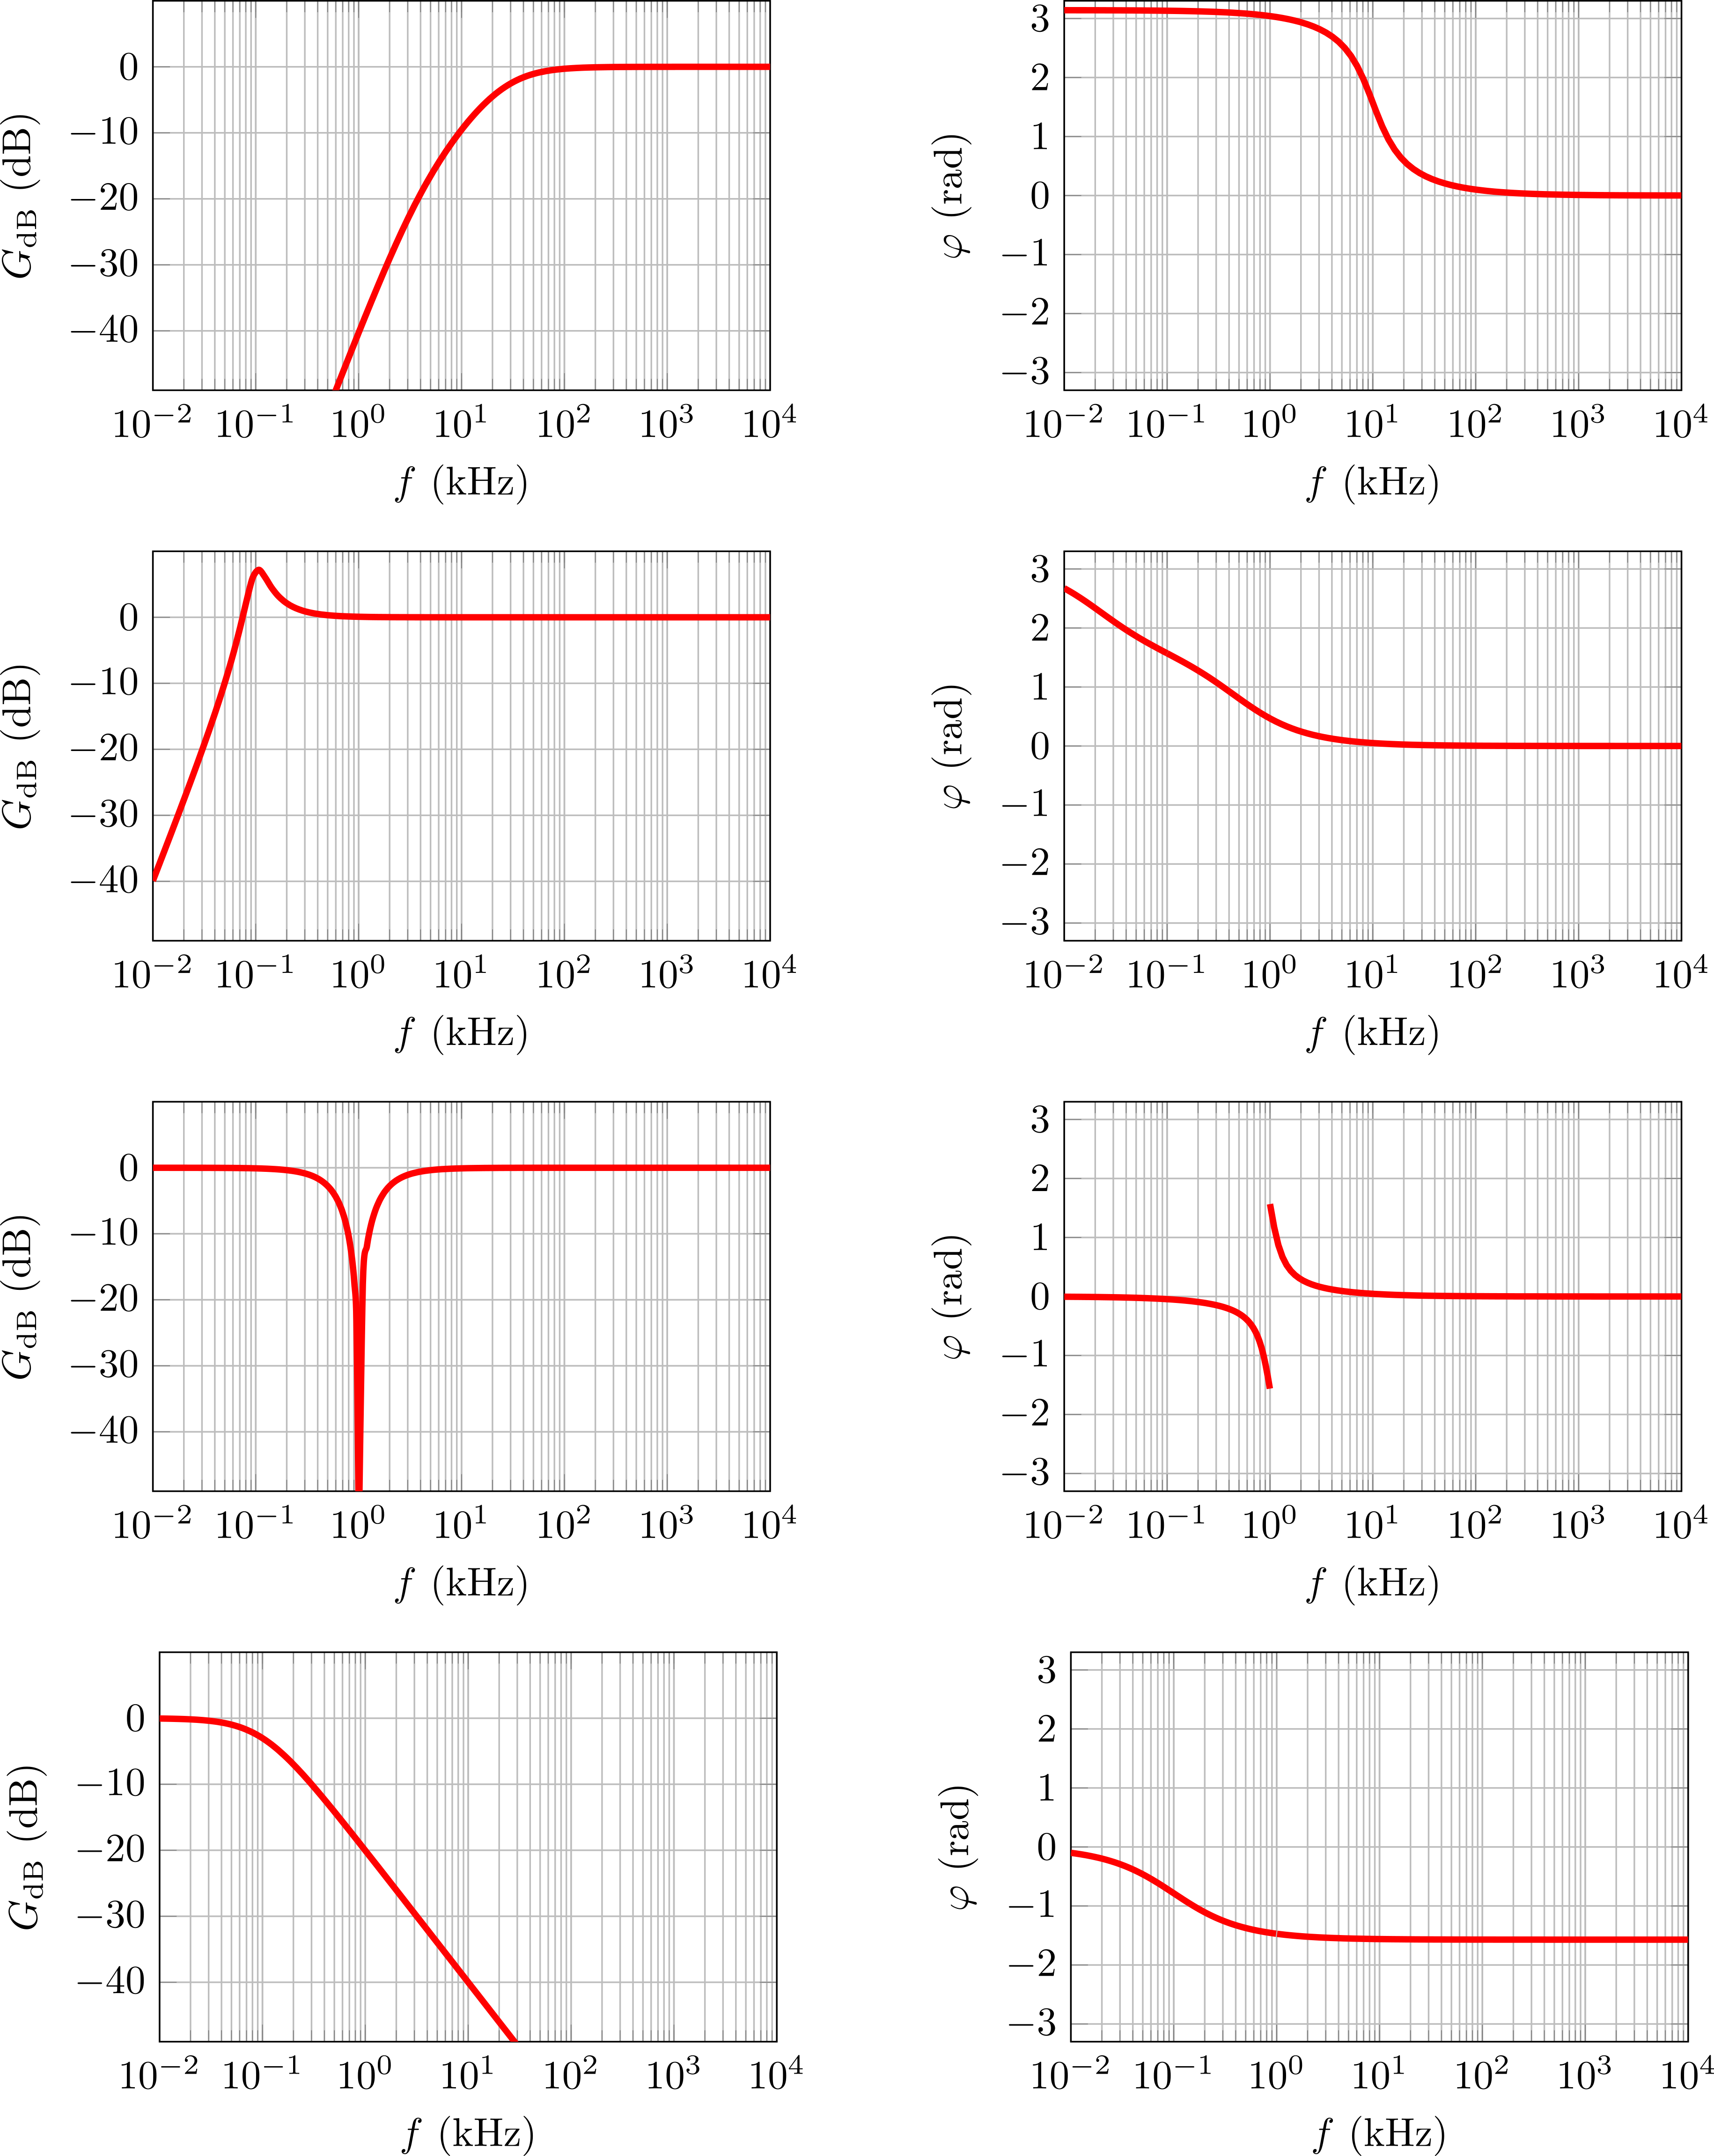
\includegraphics[scale=1]{bode_lect-plain}
		\caption{Diagrammes exercice III}
		\label{fig:ddBIII}
	\end{figure}
}
\QR{%
	Pour chacun d'eux~:
	\begin{enumerate}
		\item Indiquer le type de filtre dont il s'agit.
		\item Déterminer l'expression du signal $s(t)$ de sortie du filtre pour un
		      signal d'entrée
		      \[e(t) =
			      E_0 +
			      E_0\cos(\wt) +
			      E_0\cos \left( 10\wt + \frac{\pi}{4} \right) +
			      E_0\cos \left( 100\wt - \frac{\pi}{3} \right)
		      \]
		      avec une fréquence $f = \SI{1}{kHz}$.
	\end{enumerate}
}{%
	Pour faciliter la rédaction on note $e(t) = e_0 + e_1 (t) + e_{10} (t) + e_{100}
		(t)$, et de même pour le signal de sortie $s$. Ainsi, par linéarité, chaque
	composante $e_n$ du signal d'entrée donne une composante $s_n$ au signal de
	sortie.
	\begin{itemize}
		\item Filtre 1~: d'après l'allure du diagramme de \textsc{Bode}, il s'agit d'un
		      filtre passe-haut, de fréquence de coupure $f_c$ de l'ordre de
		      \SI{10}{kHz}. Reconstruisons le signal de sortie~:
		      \begin{itemize}
			      \item Le terme constant $e_0$ est complètement coupé par le filtre,
			            donc $s_0 = 0$.
			      \item L'harmonique de fréquence $f$ est atténuée de \SI{40}{dB} et
			            peut donc être négligée dans le signal de sortie (\SI{40}{dB}
			            correspond à une division de l'amplitude par 100), soit $s_1 (t)
				            \ll$ autres harmoniques de $s(t)$.
			      \item L'harmonique de fréquence $10f$ est atténuée de \SI{10}{dB},
			            soit \[S = 10^{-10/20} E = 10^{-1/2} E \approx \num{0,3}E\] et
			            elle est également déphasée d'environ $+\pi/2$. Ainsi \[s_{10}
				            (t) \approx \num{0,3}E \cos(10\wt + \pi/4 + \pi/2)\]
			      \item L'harmonique de fréquence $100f$ n'est presque pas atténuée ni
			            déphasée, donc $s_{100} (t) \approx e_{100} (t)$. Au final, on
			            obtient le signal de sortie $s(t)$ suivant~:
		      \end{itemize}
	\end{itemize}

	\[\boxed{
			s(t) \approx
			\num{0,3}E_0 \cos \left(10\wt + \frac{3\pi}{4}\right) +
			E_0 \cos \left(100\wt - \frac{\pi}{3}\right)
		}\]

	\begin{itemize}
		\item Filtre 2~: d'après l'allure du diagramme de \textsc{Bode}, il s'agit d'un
		      filtre \textbf{passe-haut}, de fréquence de coupure $f_c$ de l'ordre de
		      \SI{0.1}{kHz}. De la même manière que pour le fitre 1, on détermine que~:
	\end{itemize}

	\[\boxed{
			s(t) \approx
			E_0 \cos (\wt) + E_0 \cos \left(10\wt + \frac{\pi}{4}\right) +
			E_0 \cos \left(100\wt - \frac{\pi}{3}\right)
		}\]
	\begin{itemize}
		\item Filtre 3~: d'après l'allure du diagramme de \textsc{Bode}, il s'agit d'un
		      filtre \textbf{coupe-bande}, la bande coupée étant proche de
		      \SI{1}{kHz}. Ainsi seule l'harmonique $e_1(t)$ est coupée (soit $s_1 =
			      0$). Les autres composantes harmoniques du signal d'entrée, y compris la
		      composante continue, sont de fréquences suffisamment différentes de la
		      fréquence coupée pour n'être ni atténuée ni déphasée. La signal de
		      sortie $s(t)$ s'écrit donc sous la forme~:
	\end{itemize}

	\[\boxed{
			s(t) =
			E_0 +
			E_0 \cos \left(10\wt - \frac{\pi}{4}\right) +
			E_0 \cos \left(100\wt - \frac{\pi}{3}\right)
		}\]
	\begin{itemize}
		\item Filtre 4~: d'après l'allure du diagramme de \textsc{Bode}, il s'agit
		      d'un filtre \textbf{passe-bas}, de fréquence de coupure $f_c$ de l'ordre
		      de \SI{0.1}{kHz}. Le terme constant $e_0$ passe au travers du filtre
		      sans être modifié. Les termes suivants sont de fréquence suffisamment
		      supérieure à la fréquence de coupure pour que le diagramme de
		      \textsc{Bode} puisse être approximé par son asymptote. On peut alors
		      déterminer le signal de sortie comme dans le cas du premier filtre, mais
		      il y a plus simple~! Comme le filtre est d'ordre 1 (une seule asymptote
		      de pente \SI{-20}{dB/décade}, alors il se comporte comme un intégrateur
		      pour les signaux de fréquence supérieure à sa fréquence de coupure. En
		      déduire le signal de sortie est donc très simple~:
	\end{itemize}

	\[s(t) =
		E_0 +
		\frac{\w_c}{\w}E_0\sin(\wt) +
		\frac{\w_c}{10\w}\sin \left( 10\wt + \frac{\pi}{4} \right) +
		\frac{\w_c}{100\w} \sin \left( 100\wt - \frac{\pi}{3} \right)
	\]
	\begin{itemize}
		\item{}
		      En écrivant le signal en termes de cosinus, on obtient~:
	\end{itemize}
	\[\boxed{
			s(t) =
			E_0 +
			\frac{\w_c}{\w}E_0\cos\left(\wt - \frac{\pi}{2}\right) +
			\frac{\w_c}{10\w}\cos \left( 10\wt - \frac{\pi}{4} \right) +
			\frac{\w_c}{100\w} \cos \left( 100\wt - \frac{5\pi}{6} \right)
		}\]
}


\resetQ
\section{Filtre de \textsc{Wien}}
\enonce{%
	\noindent
	\begin{minipage}[c]{.3\linewidth}
		On s'intéresse au filtre de \textsc{Wien}, représenté ci-contre.
	\end{minipage}
	\hfill
	\begin{minipage}[c]{.7\linewidth}
		~
		\begin{center}
			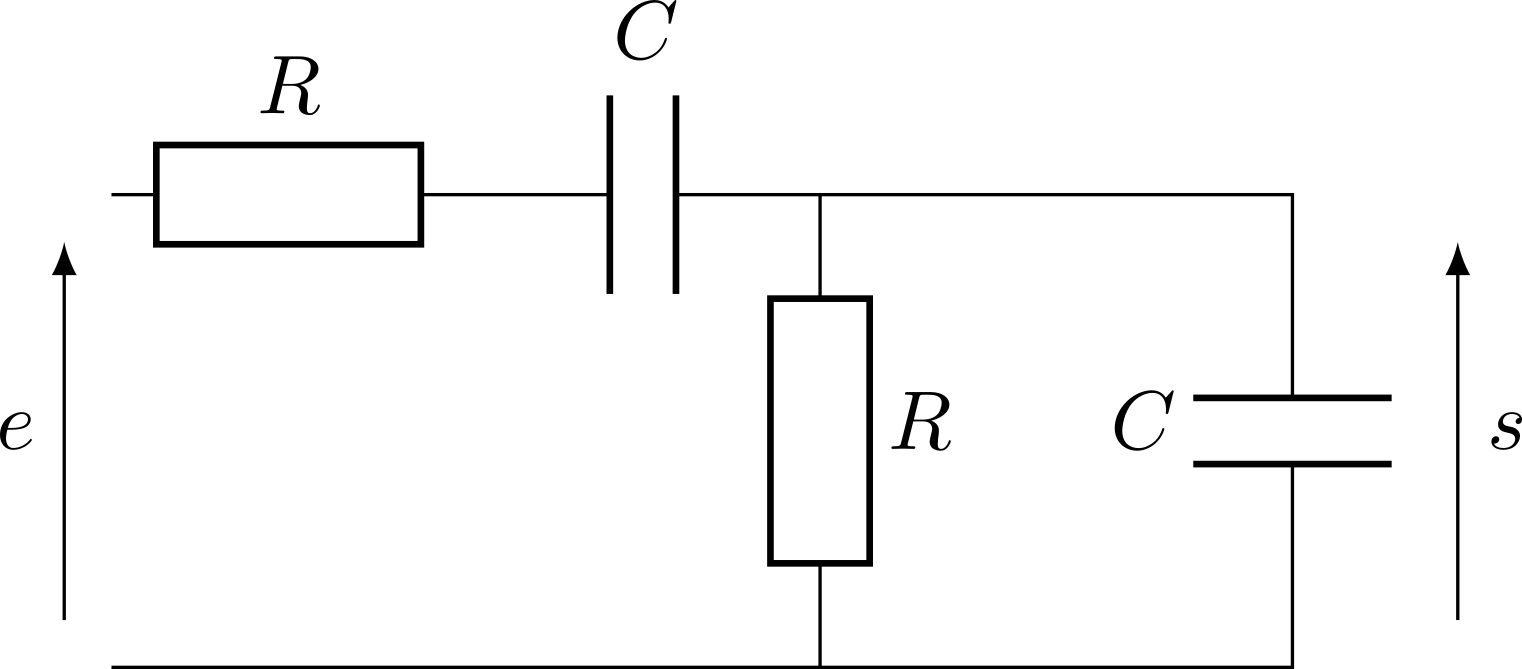
\includegraphics[width=.6\textwidth]{wien_circ-plain}
		\end{center}
	\end{minipage}
}

\QR{%
	Par analyse des comportements asymptotiques, déterminer le type de
	filtre dont il s'agit.
}{%
	Dans la limite très hautes fréquences, les condensateurs sont
	équivalents à des fils, donc $\Su = 0$. Dans la limite très basses
	fréquences, les condensateurs sont cette fois équivalents à des
	interrupteurs ouverts. Aucun courant ne circule dans les résistances, et
	on a donc également $\Su = 0$. Selon toute vraisemblance, c'est donc
	un filtre \textbf{passe-bande}.
}

\QR{%
	Déterminer la fonction de transfert $\Hu$ du filtre.
}{%
	Notons $\Zu$ l'impédance et $\Yu$ l'admittance de l'association
	RC parallèle. En utilisant cette impédance, on reconnaît un pont
	diviseur de tension~:
	\begin{gather*}
		\Hu = \frac{\Su}{\Eu} = \frac{\Zu}{R + \dfrac{1}{\jj
				C\w} + \Zu}
		\Lra
		\Hu
		= \frac{1}{1 + \left(R + \dfrac{1}{\jj C\w}\right)\Yu}
		= \frac{1}{1 + \left(R + \dfrac{1}{\jj C\w}\right)\left(
			\dfrac{1}{R} + \jj C\w\right)}\\
		\Lra
		\boxed{\Hu = \frac{1}{3+\jj\left(RC\w - \dfrac{1}{RC\w}\right)}}
	\end{gather*}
}

\QR{%
	On pose $\w_0 = 1/RC$ et $x=\w/\w_0$. Écrire la fonction de transfert
	sous la forme
	\[ \Hu = \frac{H_0}{1 + \jj Q \left( x - \dfrac{1}{x} \right)}\]
	en précisant les valeurs de $H_0$ et $Q$.
}{%
	En factorisant par 3 et en utilisant les notations introduites dans
	l'énoncé, on trouve
	\begin{gather*}
		\Hu
		= \frac{1/3}{1 + \dfrac{\jj}{3} \left( x - \dfrac{1}{x} \right)}
		\Lra
		\boxed{
			\Hu = \frac{H_0}{1 + \jj Q \left( x - \dfrac{1}{x} \right)}}
		\qavec
		\boxed{
			\left\{
			\begin{array}{rcl}
				H_0 & = & 1/3 \\
				Q   & = & 1/3
			\end{array}
			\right.
		}
	\end{gather*}
}

\QR{%
	Calculer simplement le gain maximal du filtre, puis le gain maximal en
	décibels, et le déphasage correspondant à ce maximum.
}{%
	Le gain en amplitude du filtre est défini par
	\[G = \abs{\Hu} = \frac{H_0}{\sqrt{1 + Q^2 \left( x - \dfrac{1}{x}
				\right)^2}}\]
	Il est maximal lorsque le dénominateur est minimal, c'est-à-dire lorsque
	le terme entre parenthèses s'annule. Cela correspond à $x=1$, d'où le
	gain maximal $\mathbf{G_{\max} = 1/3}$. \bigbreak
	Le gain \textbf{en décibels} du filtre est défini par
	\[G_{\rm dB} = 20\log(\abs{\Hu})\]
	et on trouve donc $\mathbf{G_{\rm dB, max} = 20\log(1/3) =
			\SI{-9.5}{dB}}$. De plus, en $x = 1$ la fonction de transfert est
	réelle, donc son argument est nul~: à la pulsation $\w_0$, la sortie et
	l'entrée ne sont donc pas déphasées.
}

\QR{%
	Représenter le diagramme de \textsc{Bode} asymptotique du filtre et en
	déduire qualitativement le tracé réel.
}{%
	Dans la limite très basses fréquences, la fonction de transfert est
	équivalente à
	\[\Hu
		\underset{x\ra0}{\sim} \frac{H_0}{-\jj Q/x}
		= \jj \frac{H_0}{Q} x
		\qdonc
		\left\{
		\begin{array}{rcl}
			G_{\dB} & = & 20\log\abs{\Hu}
			\underset{x\ra0}{\sim} 20 \log x       \\
			\f      & = & \arg \Hu = \frac{\pi}{2}
		\end{array}
		\right.
	\]
	De même, dans la limite très hautes fréquences, on a
	\[\Hu
		\underset{x\ra\infty}{\sim} \frac{H_0}{\jj Qx}
		= -\jj \frac{H_0}{Q} \frac{1}{x}
		\qdonc
		\left\{
		\begin{array}{rcl}
			G_{\dB} & = & 20\log\abs{\Hu}
			\underset{x\ra0}{\sim} -20 \log x       \\
			\f      & = & \arg \Hu = -\frac{\pi}{2}
		\end{array}
		\right.
	\]

	Ainsi, le diagramme de \textsc{Bode} asymptotique en gain compte
	\textbf{deux asymptotes de pentes $\mathbf{\pm}$ \SI{20}{dB/décade}
		passant par $\mathbf{G_{\dB} = 0}$ pour $\mathbf{x=1}$}, alors que le
	diagramme asymptotique en phase compte \textbf{deux asymptotes
		horizontales de hauteurs $\mathbf{\pm \pi/2}$}. \bigbreak
	Pour tracer l'allure du diagramme réel, on utilise en plus les résultats
	de la question précédente qui indique que la courbe réelle passe par
	$G_{\dB} = \SI{-9.5}{dB}$ en $x=1$, alors que la courbe de phase réelle
	passe par $0$ en $x=1$~; d'où les diagrammes ci-dessous.

	\begin{center}
		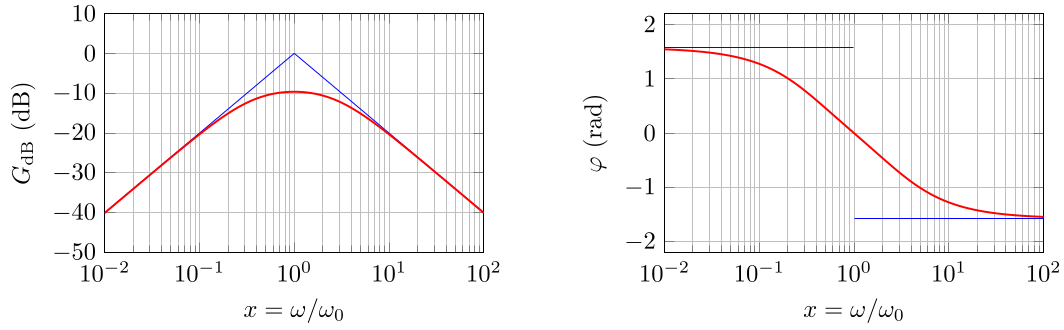
\includegraphics[width=\linewidth]{wien_bode}
	\end{center}
}

\QR{%
	Calculer la pulsation propre $\w_0$ pour $R = \SI{1.0}{k\Omega}$ et $C
		= \SI{500}{nF}$. Donner le signal de sortie du filtre si le signal
	d'entrée est
	\[e(t) = E_0 + E_0\cos(\wt) + E_0\cos(10\wt) + E_0\cos(100\wt)\]
	avec $E_0 = \SI{10}{V}$ et $\w = \SI{200}{rad.s^{-1}}$.
}{%
	Numériquement, on trouve $\w_0 = \SI{2.0e3}{rad.s^{-1}}$. Comme le
	diagramme de \textsc{Bode} réel n'est pas donné dans l'énoncé, on peut
	au choix utiliser la fonction de transfert ou raisonner sur le diagramme
	asymptotique. Étudions le signal de sortie du filtre associé à chaque
	composante du signal d'entrée~:
	\begin{itemize}
		\item Le terme continu est complètement coupé par le filtre~;
		\item Le terme de pulsation $\w = \w_0/10$ se trouve une décade
		      en-dessous de la pulsation propre~: avec le diagramme
		      asymptotique il est donc atténué de \SI{20}{dB}, ce qui
		      correspond à un facteur 10 en amplitude, et déphasé d'environ
		      \SI{1.2}{rad} si le diagramme réel tracé~;
		\item Le terme de pulsation $10\w = \w_0$ est à la pulsation propre
		      du filtre~: il n'est pas déphasé mais seulement atténué d'un
		      facteur 1/3 (gain maximal)~;
		\item Le terme à la pulsation $100\w = 10\w_0$ est une décade
		      au-dessus de la pulsation propre~: il est atténué comme le
		      premier terme d'un facteur 10 en amplitude, et déphasé d'environ
		      \SI{-1.2}{rad}. Ainsi,
	\end{itemize}
	\[\boxed{
			s(t) =
			\frac{E_0}{10}\cos (\wt - \num{1.2}) +
			\frac{E_0}{3}\cos(10\wt) +
			\frac{E_0}{10}\cos (100\wt + \num{1.2})
		}\]
}

\resetQ
\section{Filtre ADSL}
\enonce{%
	Un lutin malin semble avoir chourré votre filtre ADSL. Sale histoire.
	Heureusement, vous avez les connaissances pour en recréer un~! En sachant que
	les signaux transmis par une ligne téléphonique utilisent une très large gamme
	de fréquences, divisée en deux parties~:
	\begin{itemize}
		\item les signaux téléphoniques (transmettant la voix) utilisent les
		      fréquences de 0 à \SI{4}{kHz}~;
		\item les signaux informatiques (Internet) utilisent les fréquences de
		      \SI{25}{kHz} à \SI{2}{MHz}.
	\end{itemize}
}

\QR{%
	Quel type de filtre faut-il utiliser pour récupérer seulement les
	signaux téléphoniques~? Les signaux informa- tiques~? Quelle fréquence
	de coupure peut-on choisir~?
}{%
	On isole les signaux téléphoniques avec un \textbf{filtre passe-bas},
	et les signaux informatiques avec un \textbf{filtre passe-haut}. La
	fréquence de coupure doit être à la fois nettement supérieure aux
	fréquences téléphoniques et nettement plus faible que les fréquences
	informatiques~: on prendra donc \fbox{$f_0 = \SI{10}{kHz}$}.
}

\enonce{%
	Vous réalisez le filtre ci-dessous.
	\begin{center}
		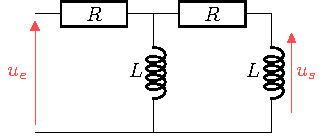
\includegraphics[width=.5\linewidth]{adsl_plain}
	\end{center}
}

\QR{%
	Déterminer la nature du filtre grâce à son comportement asymptotique
	en basses fréquences et en hautes fréquences. En déduire pour quels
	signaux il peut être utilisé.
}{%
	\begin{isd}
		En basses fréquences ($\w \lra 0$), les bobines se
		comportent comme des fils, soit
		\begin{center}
			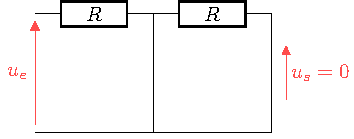
\includegraphics[width=\linewidth]{adsl_bf}
		\end{center}
		\tcblower
		En hautes fréquences ($\w \lra \infty$), les bobines se
		comportent comme des interrupteurs ouverts, soit
		\begin{center}
			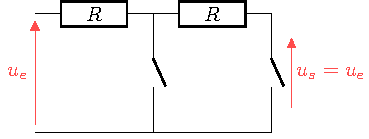
\includegraphics[width=\linewidth]{adsl_hf}
		\end{center}
	\end{isd}
	Ainsi, le signal de sortie est non nul pour les hautes fréquences, et
	négligeable pour les basses fréquences~: c'est un \textbf{filtre
		passe-haut}. Il permettra d'obtenir les signaux informatiques.
}

\QR{%
	Montrer que la fonction de transfert de ce filtre peut se mettre sous
	la forme~:
	\[\Hu(x) = \frac{-x^2}{1 + 3\jx-x^2}
		\qavec
		x = \frac{\w}{\w_0}
	\]
	et exprimer $\w_0$ en fonction de $R$ et $L$.
}{%
	Pour exprimer $u_s$ en fonction de $u_e$, on peut faire un premier
	pont diviseur de tension pour exprimer $u_s$ en fonction de $u_{AB}$ du
	milieu~; puis avec une impédance équivalente à l'ensemble des 3 dipôles
	de droite, on refait un pont diviseur de tension pour avoir $u_{AB}$ en
	fonction de $u_e$, et on combine.
	\begin{center}
		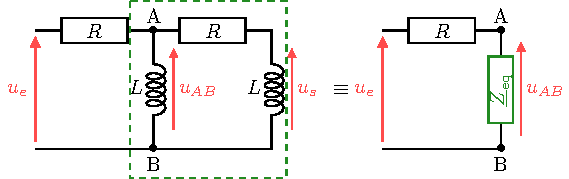
\includegraphics[width=0.8\linewidth]{adsl_equiv}
	\end{center}
	On a donc d'abord~:
	\begin{gather*}
		\Uu_s = \frac{\Zu_L}{\Zu_L + \Zu_R}\Uu_{AB}
		\Lra
		\Uu_s = \frac{\jlw}{\jlw + R}\Uu_{AB}
	\end{gather*}
	On aura donc ensuite~:
	\begin{gather*}
		\Uu_{AB} = \frac{\Zu\ind{eq}}{\Zu\ind{eq} + \Zu_R}\Uu_e
		\Lra
		\Uu_{AB} = \frac{1}{1+\Zu_R\Yu\ind{eq}}\Uu_e
	\end{gather*}
	On calcule alors $\Yu\ind{eq}$~:
	\begin{gather*}
		\Yu\ind{eq} = \frac{1}{\jlw} + \frac{1}{R+\jlw}
	\end{gather*}
	Et on combine~:
	\begin{gather*}
		\Uu_s =
		\frac{\jlw}{R+\jlw}\times\frac{1}{1+\Zu_R\Yu\ind{eq}}\Uu_e
		\Lra
		\Uu_s =
		\frac{\jlw}{R + \jlw + R \left( \dfrac{R+\jlw}{\jlw} + 1
			\right)}\times {\color{Red} \frac{\jlw}{\jlw}}\Uu_e\\
		\Lra
		\Uu_s =
		\frac{-(L\w)^2}{R^2 + 3\jj RL\w - (L\w)^2}\Uu_e
		\Lra
		\Uu_s =
		{\color{red}\cancel{\frac{R^2}{R^2}}}
		\frac{- \left( \dfrac{L}{R}\w \right)^2}{1 + 3\jj \dfrac{L}{R}\w
			- \left( \dfrac{L}{R}\w \right)^2}
		\Uu_e
	\end{gather*}
	Ainsi, en divisant par $\Uu_e$ pour avoir la fonction de transfert, on
	a~:
	\begin{gather*}
		\boxed{\Hu = \frac{-x^2}{1-x^2+3\jx}}
		\qavec
		\boxed{\w_0 = \frac{R}{L}}
	\end{gather*}
}

\QR{%
	Tracer le diagramme de Bode asymptotique (gain et phase) de ce filtre,
	puis esquisser l'allure de la courbe réelle de gain en la justifiant.
}{%
	Pour $x \gg 1$, les termes en $x^2$ l'emportent sur les autres termes
	au numérateur et au dénominateur, et la fonction de transfert devient
	$\Hu \underset{x\ra\infty}{\sim} 1$, donc \fbox{$G_{\dB} = 0$}
	et \fbox{$\f = 0$} (réel positif). \bigbreak
	Pour $x \ll 1$, les termes en $x$ sont négligeables devant $1$ au
	dénominateur, et on garde le numérateur~: la fonction de transfert
	devient donc $\Hu \underset{x\ra0}{\sim} -x^2$, donc
	\fbox{$G_{\dB} \underset{x\ra0}{\sim} 40\log(x)$} (pente de
	\SI{40}{dB/décade}), et \fbox{$\f = -\pi$} (réel négatif). \bigbreak
	Pour $x = 1$, on trouve $\Hu(1) = \jj/3$ donc \fbox{$G_{\dB}(1) =
			20\log(1/3) = \SI{-9.5}{dB}$}, et \fbox{$\f(1) = \pi/2$} (imaginaire pur).
	\begin{center}
		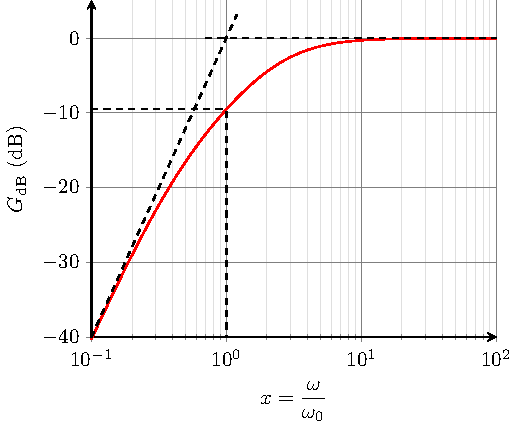
\includegraphics[width=.48\linewidth]{adsl_bode-gain}
		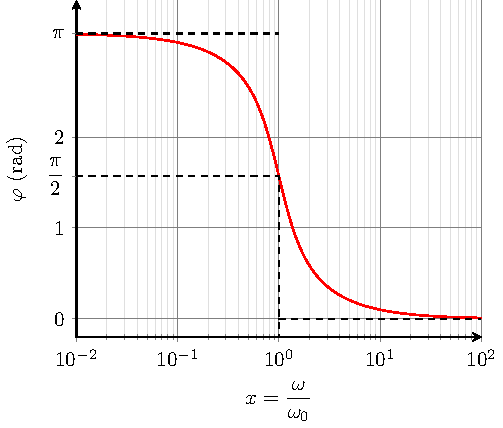
\includegraphics[width=.48\linewidth]{adsl_bode-phase}
	\end{center}
	Il n'y a pas de pic de résonance car le facteur de qualité $Q$ est
	plus petit que $1/\sqrt{2}$.
}

\QR{%
	Vous possédez des résistances de $\SI{100}{\Omega}$. Quelle valeur
	d'inductance $L$ choisir pour réaliser le filtre souhaité~?
}{%
	La fréquence de coupure est $f_0 = \DS \frac{\w_0}{2\pi} =
		\frac{R}{2\pi L}$~; on doit donc prendre
	\begin{gather*}
		\boxed{L = \frac{R}{2\pi f_0}}
		\qavec
		\left\{
		\begin{array}{rcl}
			R   & = & \SI{100}{\Omega} \\
			f_0 & = & \SI{10}{kHz}
		\end{array}
		\right.\\
		\mathrm{A.N.~:}\quad
		\boxed{L = \SI{1.6}{mH}}
	\end{gather*}
}

\resetQ
\section{Filtre de \textsc{Colpitts}}

\enonce{%
	\noindent
	\begin{minipage}{.50\linewidth}
		On considère le quadripôle suivant, où $C$ est une capacité, $R$ une
		résistance et $L$ une inductance. Il est utilisé en régime sinusoïdal forcé
		de pulsation $\w$, en sortie «~ouverte~» (rien n'est branché aux bornes de
		sortie).
	\end{minipage}
	\begin{minipage}{0.50\linewidth}
		\begin{center}
			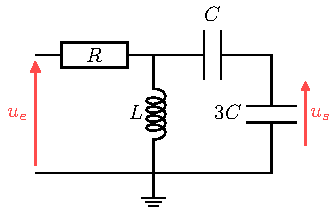
\includegraphics[width=.8\linewidth]{colpitts_plain}
		\end{center}
	\end{minipage}
}

\QR{%
	Étudier qualitativement le comportement de ce quadripôle en hautes et
	basses fréquences. De quel type de filtre s'agit-il~?
}{%
	~

	\vspace{-18pt}
	\begin{minipage}{0.48\linewidth}
		En basses fréquences ($\w \ra 0$), les condensateurs se
		comportent comme des interrupteurs ouverts, la bobine comme un fil~: la
		tension $u_s$ est donc nulle.
		\begin{center}
			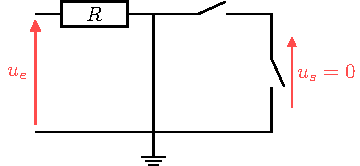
\includegraphics[width=\linewidth]{colpitts_bf}
		\end{center}
	\end{minipage}
	\hfill
	\vrule
	\hfill
	\begin{minipage}{0.48\linewidth}
		En hautes fréquences ($\w \ra \infty$), les condensateurs se
		comportent comme des fils, la bobine comme un interrupteur ouvert~: la
		tension $u_s$ est donc nulle.
		\begin{center}
			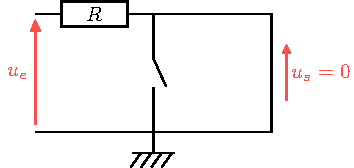
\includegraphics[width=\linewidth]{colpitts_hf}
		\end{center}
	\end{minipage}

	Comme la tension est nulle aux extrêmes, c'est un \textbf{passe-bande}.
	Si elle était égale à la tension d'entrée aux extrêmes, ça serait un
	coupe-bande.
}

\QR{%
	Déterminer la fonction de transfert $\Hu(\jw) =
		\dfrac{\xul{u_s}}{\xul{u_e}}$ et la mettre sous l'une des formes
	équivalentes~:
	\[\Hu(\jw) = \frac{A}{1+\jj Q \left( \dfrac{\w}{\w_0} -
			\dfrac{\w_0}{\w} \right)} = \frac{\jj\dfrac{A}{Q}\dfrac{\w}{\w_0}}{1
			- \dfrac{\w^2}{\w_0{}^2} + \dfrac{\jj}{Q} \dfrac{\w}{\w_0}}\]
	En introduisant des constantes $A$, $w_0$ et $Q$ dont on précisera les
	expressions en fonction de $R$, $L$ et $C$.
}{%
	On effectue deux diviseurs de tension successifs~: un pour déterminer
	$u_s$ en fonction de $u_L$, puis avec une impédance équivalente des
	trois dipôles de droite, on détermine $u_L$ en fonction de $u_e$ et on
	combine. C'est le même fonctionnement que pour l'exercice sur l'ADSL,
	question 3.
	\begin{center}
		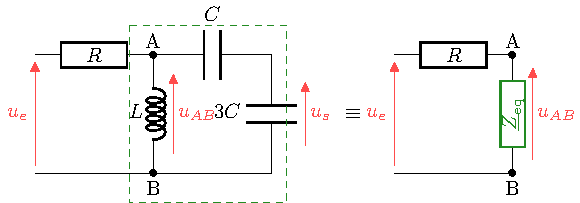
\includegraphics[width=0.8\linewidth]{colpitts_equiv}
	\end{center}
	On a ainsi en premier lieu
	\begin{gather*}
		\Uu_s = \frac{\Zu_{3C}}{\Zu_{3C} + \Zu_C}\Uu_{AB}
		\Lra
		\Uu_s = \frac{1/\jj3C\w}{1/\jj3C\w + 1/\jj C\w}\Uu_{AB}
		\Lra
		\Uu_s = \frac{1}{1+3}\Uu_{AB}
		\Lra
		\boxed{\Uu_s = \frac{\Uu_{AB}}{4}}
	\end{gather*}
	On aura donc ensuite~:
	\begin{gather*}
		\Uu_{AB} = \frac{\Zu\ind{eq}}{\Zu\ind{eq} + \Zu_R}\Uu_e
		\Lra
		\boxed{\Uu_{AB} = \frac{1}{1+\Zu_R\Yu\ind{eq}}\Uu_e}
	\end{gather*}
	On calcule alors $\Yu\ind{eq}$ de l'association en parallèle de $L$ et
	$C$ en série avec $3C$. \textbf{Attention} à l'association en série de
	capacités~:
	\begin{gather*}
		Z_{C+3C} = \frac{1}{\jj3C\w} + \frac{1}{\jcw}{\color{orange}\times
			\frac{3}{3}} = \frac{4}{\jj3C\w}\\
		\Yu\ind{eq} = \Yu_L + \Yu_{C+3C}
		\Lra
		\boxed{\Yu\ind{eq} = \frac{1}{\jlw} + \jj3C\w/4}
	\end{gather*}
	Et on combine~:
	\begin{gather*}
		\Uu_s =
		\frac{1}{4}
		\frac{1}{1+R \left( \dfrac{1}{\jlw} + \dfrac{\jj3C\w}{4} \right)}
		\Uu_e
		\Lra
		\Uu_s =
		\frac{1}{4}
		\frac{1}{1+\jj \left( - \dfrac{R}{L\w} + \dfrac{3RC\w}{4} \right)}
		\Uu_e
		\\
	\end{gather*}
	Ainsi, en divisant par $\Uu_e$ pour avoir la fonction de transfert, on
	a~:
	\begin{gather*}
		\Hu = \frac{1/4} {1+\jj\left(\dfrac{3RC\w}{4}-\dfrac{R}{L\w}\right)}
		\Lra
		\boxed{\Hu = \frac{A}{1+\jj Q \left( \dfrac{\w}{\w_0} -
				\dfrac{\w_0}{\w} \right)}}
		\qavec
		\boxed{A = \frac{1}{4}}
	\end{gather*}
	Reste à trouver $Q$ et $\w_0$. Pour cela, on identifie membre à membre~:
	\begin{align*}
		\frac{Q}{\w_0} = \frac{3RC}{4} \quad (1)
		 & \qet
		Q\w_0 = \frac{R}{L} \quad (2) \\
		\Lra
		\boxed{Q = \frac{R\sqrt{3C}}{2\sqrt{L}}}
		 & \qet
		\boxed{\w_0 = \frac{2}{\sqrt{3LC}}}
	\end{align*}
	où l'on obtient $Q$ et $\w_0$ en multipliant les équations (1) et (2)
	d'une part puis en en prenant la racine carrée, et en divisant (2) par
	(1) en en prenant la racine carrée, respectivement.
}
\enonce{%
	Le diagramme de \textsc{Bode} de ce quadripôle pour $Q = 6$ est donné
	ci-dessous.
	\begin{center}
		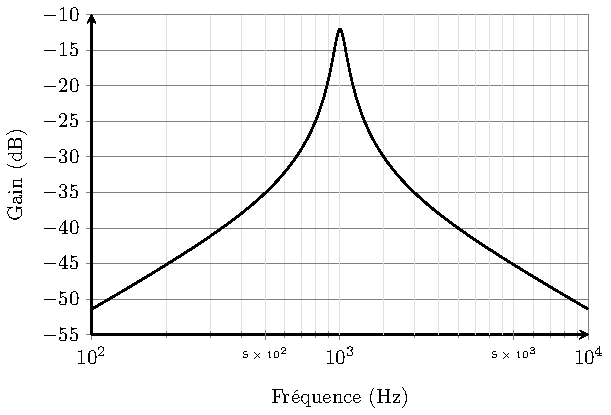
\includegraphics[width=.46\linewidth]{colpitts_bode-gain}
		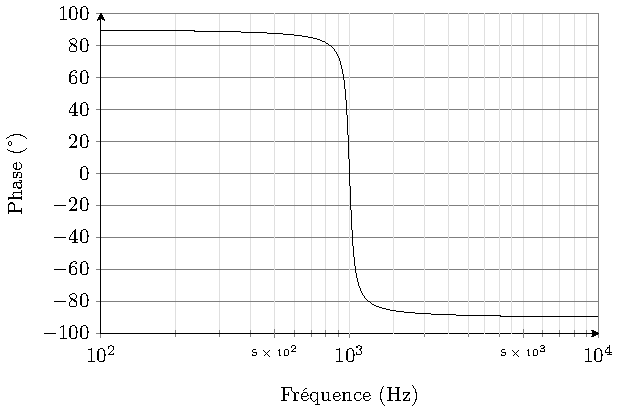
\includegraphics[width=.46\linewidth]{colpitts_bode-phase}
	\end{center}
}

\QR{%
	Justifier l'allure des parties rectilignes du diagramme.
	Déduire du diagramme la valeur de la fréquence d'accord $f_0 =
		\w_0/2\pi$ ainsi que des fréquences de coupure.
}{%
	Les parties rectilignes du diagramme correspondent aux limites
	asymptotiques du gain en décibels, c'est-à-dire pour $\w \ll \w_0$ et
	$\w \gg \w_0$. En effet,
	\begin{align*}
		\Hu \underset{\w \ll \w_0}{\sim} \jj \frac{A}{Q} \frac{\w}{\w_0}
		 & \qet
		\Hu \underset{\w \gg \w_0}{\sim} -\jj \frac{A}{Q} \frac{\w_0}{\w}
		\\
		\Lra
		G_{\dB} \underset{\w \ll \w_0}{\sim}
		20 \log \frac{A}{Q} + 20 \log \frac{\w}{\w_0}
		 & \qet
		G_{\dB} \underset{\w \gg \w_0}{\sim}
		20 \log \frac{A}{Q} - 20 \log \frac{\w}{\w_0}
		\\
		\Lra
		\f \underset{\w \ll \w_0}{\sim} \frac{\pi}{2}
		 & \qet
		\f \underset{\w \gg \w_0}{\sim} - \frac{\pi}{2}
	\end{align*}
	Pour $\w = \w_0$, on trouve simplement $\Hu = A$ donc $G_{\dB}(\w_0) =
		\SI{-12}{dB}$ et $\f = 0$. La fréquence de résonance (ou fréquence d'accord)
	correspond au pic du diagramme de \textsc{Bode} (ou à l'intersection des
	asymptotes du gain en décibels) d'une part, ou correspond à la fréquence
	pour laquelle la phase est nulle~: on lit simplement \fbox{$f_0 =
			\SI{1}{kHz}$}. \bigbreak
	On trouve les fréquences de coupure en trouvant les fréquences $f_1$ et
	$f_2$ telles que $G_{\dB} = G_{\max} - \SI{3}{dB}$, soit $G_{\dB} =
		\SI{-15}{dB}$~: on lit approximativement \fbox{$f_1 = \SI{950}{Hz}$} et
	\fbox{$f_2 = \SI{1050}{Hz}$}.
}


\resetQ
\section{Filtre de \textsc{Butterworth} d'ordre 3}
\enonce{%
	On veut réaliser un filtre de \textsc{Butterworth} d'ordre 3, dont le module $H$
	de sa fonction de transfert harmonique en tension $\Hu$ s'exprime~:
	\[H = \abs{\Hu} = \sqrt{\frac{1}{1+\left(\dfrac{\w}{\w_0}\right)^6}} =
		\sqrt{\frac{1}{1+x^6}}
		\qavec
		x = \frac{\w}{\w_0}
	\]
}

\QR{%
	Montrer qu'une fonction de transfert $\Hu = \DS \frac{1}{1+2\jx +
			2(\jx)^2 + (\jx)^3}$ correspond bien à un filtre de
	\textsc{Butterworth} d'ordre 3.
}{%
	Il suffit pour cette question de développer les puissances sur les
	$\jj$, de calculer le module et de développer~:
	\begin{gather*}
		\Hu = \left( 1 + 2\jx - 2x^2 -\jx^3 \right)^{-1}
		\Lra
		\abs{\Hu}
		= \left( (1-2x^2)^2 + (2x - x^3)^2 \right)^{-1/2}\\
		\Lra
		\abs{\Hu}
		= \left( 1-\bcancel{4x^2} + \cancel{4x^4}
		+ \bcancel{4x^2} - \cancel{4x^4} + x^6 \right)^{-1/2}
		= \left( 1+x^6 \right)^{-1/2}
	\end{gather*}
	ce qui correspond bien à un filtre de \textsc{Butterworth} d'ordre 3.
}

\QR{%
	Étudier et représenter le diagramme de \textsc{Bode} asymptotique en
	amplitude de cette fonction de transfert.
}{%
	~

	\vspace{-24pt}
	\begin{minipage}{0.48\linewidth}
		Pour étudier le diagramme de \textsc{Bode} asymptotique, on définit
		d'abord le gain en décibels~: $G_{\dB} = 20\log(\abs{\Hu}) =
			20\log(\left( 1+x^6 \right)^{-1/2}) = -10\log(1+x^6)$. Ensuite, on
		étudie son comportement asymptotique pour $x \ll 1$ et $x \gg 1$~:
		on trouve
		\begin{gather*}
			\boxed{G_{\dB} \underset{x \ll 1}{\sim} 0}
			\qet
			\boxed{G_{\dB} \underset{x \gg 1}{\sim} -60\log(x)}
		\end{gather*}
		d'où le diagramme de \textsc{Bode} asymptotique ci-contre. Par
		rapport à de l'ordre 1 (\SI{-20}{dB/décade}) ou de l'ordre 2
		(\SI{-40}{dB/décade}), l'atténuation des hautes fréquences est
		encore plus prononcé~: une fréquence 10 fois supérieure à $f_0$
		serait atténuée d'un facteur 1000 au lieu d'un facteur 10.
	\end{minipage}
	\hfill
	\begin{minipage}{0.48\linewidth}
		\begin{center}
			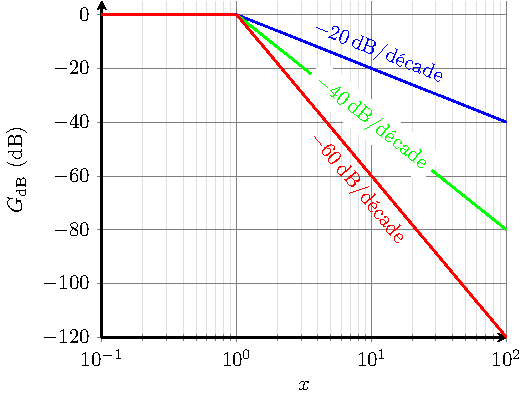
\includegraphics[width=\linewidth]{butterworth_bode-gain}
		\end{center}
	\end{minipage}
}

\QR{%
	On considère le quadripôle ci-dessous~:
	\begin{center}
		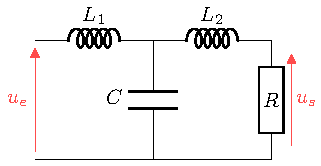
\includegraphics[width=0.5\linewidth]{butterworth_filtre-plain}
	\end{center}
	Calculer en fonction de $R$ et $\w_0$, les valeurs de $L_1$, $L_2$ et
	$C$ pour que ce filtre soit un filtre de \textsc{Butterworth} d'ordre 3.
}{%
	Ici encore, on utilise deux ponts diviseurs de tension successifs~: on
	calcule $u_s$ en fonction de $u_{AB}$, puis $u_{AB}$ en fonction de
	$u_e$ après avoir déterminé l'impédance équivalente de l'ensemble des
	dipôles de droite.
	\begin{center}
		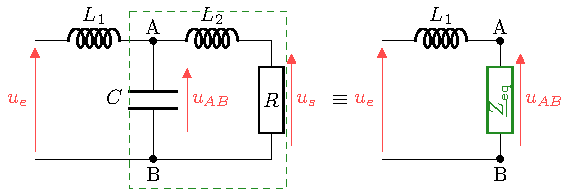
\includegraphics[width=0.8\linewidth]{butterworth_equiv}
	\end{center}
	On aura donc en premier lieu
	\begin{gather*}
		\Uu_s = \frac{\Zu_R}{\Zu_R + \Zu_{L_2}}\Uu_{AB}
		\Lra
		\boxed{\Uu_s = \frac{R}{R+\jj L_2\w}\Uu_{AB}}
	\end{gather*}
	Et ensuite, on aura
	\begin{gather*}
		\Uu_{AB} = \frac{\Zu\ind{eq}}{\Zu\ind{eq} + \Zu_{L_1}}\Uu_e
		\Lra
		\boxed{\Uu_{AB} = \frac{1}{1+\Zu_{L_1}\Yu\ind{eq}}\Uu_e}
	\end{gather*}
	On calcule alors $\Yu\ind{eq}$ de l'association en parallèle de $C$ et
	$L_2$ en série avec $R$~:
	\begin{gather*}
		Z_{L_2+R} = \jj L_2\w + R\\
		\Yu\ind{eq} = \Yu_C + \Yu_{L_2+R}
		\Lra
		\Yu\ind{eq} = \jcw + \frac{1}{\jj L_2\w + R}
		\Lra
		\Yu\ind{eq} = \frac{\jcw (\jj L_2\w + R)+1}{\jj L_2\w + R}\\
		\Lra
		\boxed{\Yu\ind{eq} = \frac{1-L_2C\w^2 + \jj RC\w}{R + \jj L_2\w}}
	\end{gather*}
	Et on combine~:
	\begin{align*}
		\Uu_s & =
		\frac{R}{R+\jj L_2\w} \times
		\frac{1}{1+\jj L_1\w
			\left( \dfrac{1-L_2C\w^2 + \jj RC\w}{R + \jj L_2\w} \right)}
		\Uu_e                                                            \\
		\Lra
		\Uu_s & =
		\frac{R}{R+\jj L_2\w}\times
		\frac{1}{1+\dfrac{\jj L_1\w - \jj L_1L_2C\w^3 + (\jj\w)^2RCL_1}
			{R + \jj L_2\w}}
		\Uu_e                                                            \\
		\Lra
		\Uu_s & =
		\frac{R}
		{R+\jj L_2\w + \jj L_1\w - \jj L_1L_2C\w^3 + (\jj\w)^2RCL_1}
		\Uu_e                                                            \\
		\Lra
		\Uu_s & = \frac{1}{1+ \jj\w \dfrac{L_1+L_2}{R} + (\jj\w)^2L_1C +
			(\jj\w)^3 \dfrac{L_1L_2C}{R}}
		\Uu_e
	\end{align*}
	en utilisant que $-\jj = \jj^3$. Ainsi, en divisant par $\Uu_e$ pour
	avoir la fonction de transfert, on a bien
	\begin{gather*}
		\boxed{\Hu = \frac{1}{1+2\jx + 2(\jx)^2 + (\jx)^3}}
		\qavec
		\left\{
		\begin{array}{rcl}
			\dfrac{2}{\w_0}     & = & \dfrac{L_1+L_2}{R} \\[12pt]
			\dfrac{2}{\w_0{}^2} & = & L_1C               \\[12pt]
			\dfrac{1}{\w_0{}^3} & = & \dfrac{L_1L_2C}{R}
		\end{array}
		\right.
		\Lra
		\boxed{
			\left\{
			\begin{array}{rcl}
				L_1 & = & \dfrac{3R}{2\w_0} \\[12pt]
				L_2 & = & \dfrac{R}{2\w_0}  \\[12pt]
				C   & = & \dfrac{4}{3Rw_0}
			\end{array}
			\right.}
	\end{gather*}
}

\QR{%
	Justifier que l'on puisse réaliser le filtre de \textsc{Butterworth}
	d'ordre 3 en associant en cascade un filtre d'ordre 1 et un filtre
	d'ordre 2, comme sur le circuit suivant~:
	\begin{center}
		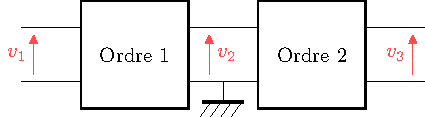
\includegraphics[width=0.6\linewidth]{butterworth_filtre_cascade-plain}
	\end{center}
	Préciser la valeur du facteur de qualité du filtre d'ordre 2.
}{%
	Pour mettre des filtres en cascade et avoir $\Hu = \Hu_1\Hu_2$, il
	faut que l'impédance de sortie du filtre 1 soit faible devant
	l'impédance d'entrée du filtre 2. Dans ce cas, on utilise un filtre
	d'ordre 1 avec un numérateur constant (donc un passe-bas de la forme
	$\Hu_1 = \frac{H_1}{1 + \jx}$), et un filtre
	d'ordre 2 avec un numérateur lui aussi constant~: soit un passe-bas soit
	un passe-bande. Le passe-bande fait intervenir $\jj Q \left( x -
		\frac{1}{x} \right)$ au dénominateur, donc il est plus simple d'utiliser
	une passe-bas d'ordre 2 avec $1 + \jj/Q x + (\jx)^2$ au dénominateur~:
	\begin{gather*}
		\Hu
		= \frac{H_1}{1+ \jx}\times \frac{H_2}{1 + \dfrac{\jj}{Q}x +
			(\jx)^2}
		= \frac{H_1H_2}{1 + \jx \left( 1 + \dfrac{1}{Q} \right)
			+ (\jx)^2 \left( 1 + \dfrac{1}{Q^2} \right) + (\jx)^3}
	\end{gather*}
	Pour trouver un filtre de \textsc{Butterworth} d'ordre 3 de cette
	manière, il faut donc $H_1 = H_2 = 1$ et \fbox{$Q = 1$}.
}


\end{document}
